In this chapter, we present a novel approach to the problem of frontier
detection. The \FFD algorithm (Section \ref{section:ffd}) avoids searching
for frontiers both in known and unknown regions of the map; it only searches
within the boundary between them. This significantly reduces the search area.
However, the search-space reduction forces \FFD to run in the background
persistently. In order to be robust against map orientation changes caused by
loop closures, \FFD has to perform maintenance over previously detected
frontiers (Section
\ref{section:ffd_maintaining_previously_detected_frontiers}). At the end of
this chapter, we prove that \FFD is complete and sound (Section
\ref{section:ffd_sound_and_complete}).

\section{Fast Frontier Detector}
\label{section:ffd}
% We propose a novel approach for frontier detection
Unlike other frontier detection methods (including \emph{WFD}), our proposed
algorithm (Algorithm \ref{alg:ffd_outline}) only processes new laser
readings which are received in real time. It therefore avoids searching both
known and unknown regions. In doing this, we make use of the fact that by
definition, frontiers represent the boundaries between the known and unknown
regions of the environment (see Figure~\ref{fig:frontiers}). Hence, scanning all
unknown regions is definitely unnecessary and not time-efficient. The \FFD
algorithm contains four steps (Algorithm \ref{alg:ffd_outline}), and
can be called with every new scan.

\begin{algorithm}[htbp]
\caption{Fast Frontier Detector (FFD): Outline}
\label{alg:ffd_outline}
\begin{algorithmic}[1]

\Require $frontiersDB$ 
\Comment{data-structure that contains last known frontiers}

\Require{$pose$} \Comment{current global position of the robot}
\Require{$lr$} \Comment {laser readings which were received in
current iteration. Each element is a 2-d cartesian point} 
\Require $activeArea$
\Comment{data-structure that contains all points that lie inside the active
area}

\Statex {\\}
%%%%%%%%%%%%%%%%%%%%%%%%%%%%%%%%%%%%%%%%%%%%%%%%%%%%%%%%%%%%%%%
\Comment{polar sort readings according to robot position}
\State $sorted \gets$ \Call {Sort-Polar}{$lr, pose$} 
\label{mark:ffd_sort}

%%%%%%%%%%%%%%%%%%%%%%%%%%%%%%%%%%%%%%%%%%%%%%%%%%%%%%%%%%%%%%%%
\Statex{\\}
\Comment{get the contour from laser readings}
\State $contour \gets$\Call {Contour}{$sorted$}
%%%%%%%%%%%%%%%%%%%%%%%%%%%%%%%%%%%%%%%%%%%%%%%%%%%%%%%%%%%%%%%%%%

\Statex{\\}
\Comment{extract new frontiers from contour}
\State $NewFrontiers \gets$ \Call {Extract-Frontiers-1D}{$contour$}

\Statex{\\}
\Comment{maintainance of previously detected frontiers}
\State \Call {Maintain-Frontiers}{$NewFrontiers,frontiersDB,activeArea$}

\end{algorithmic}
\end{algorithm}




%\begin{description}
  %\item[(1) Sorting]
  \begin{algorithm}[htbp]
\caption{Fast Frontier Detector (FFD): Sorting Stage}
\label{alg:ffd_sorting_stage}
\begin{algorithmic}[1]

\Require {$lr$} 
\Comment{set of laser readings}
\Require {$pose$} 
\Comment{current robot position}
\Ensure {$sorted$} 
\Comment{sorted laser readings according to polar coordinates}
%%%%%%%%%%%%%%%%%%%%%%%%%%%%%%%%%%%%%%%%%%%%%%%%%%%%%%%%%%%%%%%%
%\Statex{\\}
\Function{Polar-Sort}{$lr,pose$}
	\State $sorted \gets \emptyset$
	\State $A_r \gets \emptyset$
	
	
	\Comment{set robot position as origin}
	\ForAll {Point $p \in lr$}
		\State $A_r \gets polar \cup \left\{\term{p.x-pose,x, p.y-pose.y}\right\}$
	\EndFor
	
	\State $sorted \gets$ \Call{Sort}{$A_r$, \textsc{polarComparator}}
	\State \Return $sorted$
\EndFunction 
\Statex{}
\Function{polarComparator}{$p_1,p_2$}
	\State $s \gets \term{p_1.x\cdot p_2.y - p_2.x\cdot p_1.y}$
	\Comment{calculate cross-product of input points}
	\If {$s > 0$}
	\Comment{check the sign of the cross-proudct}
		\State \Return 1
	\ElsIf {$s < 0$}
		\State \Return -1
	\Else
		\State \Return 0 
	\EndIf
\EndFunction
%%%%%%%%%%%%%%%%%%%%%%%%%%%%%%%%%%%%%%%%%%%%%%%%%%%%%%%%%%%%%%%%%%
\end{algorithmic}
\end{algorithm}
  \subsection{Sorting} 
	The first step (Algorithm \ref{alg:ffd_sorting_stage}) sorts range readings
	based on their angle, i.e., based on the ego-centric polar coordinates with the robot as the origin.
	Normally, laser readings are given as a sorted set of polar coordinated points, making this
        sorting step unnecessary. However, if this is not the
	case, a sorting is needed to be applied on the received laser readings.
	
	In this case, we assume that range readings are a set of Cartesian coordinated
	points, which consists of the locations of range hits ($ \big\{
	(x_0, y_0), \ldots, (x_n, y_n) \big\}$ where $n$ is the number of readings).
	The naive method for converting Cartesian to polar coordinates
	uses two CPU time-consuming functions: \emph{atan2} and \emph{sqrt}.

	To speed angle sorting, we use a cross product~\cite{Cormen2001} to avoid converting
        Cartesian to polar coordinates, while still sorting the points based on polar angle.
	Given 3 Cartesian coordinated points: 
% 	\vspace{-7pt}
	$$P_0 =(x_0, y_0), P_1 =(x_1, y_1), P_2 =(x_2, y_2)$$  
	the \emph{cross product} is defined as: 
% \vspace{-7pt}
	$$(p_1 - p_0) \times (p_2 -p_0) =
	(x_1-x_0)\cdot(y_2-y_0)-(x_2-x_0)\cdot(y_1-y_0)$$  
	If the result is positive, then $\overrightarrow{P_0P_1}$ is clockwise from
	$\overrightarrow{P_0P_2}$. Else, it is counter-clockwise. If the result is 0,
	then the two vectors lie on the same line in the plane (i.e., the angle is the same).
	
	Therefore, by examining the sign of the cross product, we can determine the
	order of the Cartesian points according to polar coordinates, without
	calculating their actual polar coordinate value. This applies only five
	subtractions and two multiplications which are far less time-consuming than
	calling \emph{atan2} and \emph{sqrt}.	

	
\begin{algorithm}[htbp]
\caption{Fast Frontier Detector (FFD): Contour Stage}
\label{alg:ffd_contour_stage}
\begin{algorithmic}[1]

\Require {$sorted$} 
\Comment{sorted set of laser readings}
\Ensure {$contour$} 
\Comment{the contour built from the sorted laser readings}
%%%%%%%%%%%%%%%%%%%%%%%%%%%%%%%%%%%%%%%%%%%%%%%%%%%%%%%%%%%%%%%%
%\Statex{\\}
\Function{Contour}{$sorted$}
\State{$prev \gets$ \Call {Pop}{$sorted$}}
\label{mark:ffd_contour_start}
\State{$contour \gets \emptyset$}

\ForAll {Point $curr \in sorted$}
	\State {$line \gets$ \Call {Get-Line}{$prev, curr$}} 

	\ForAll {Point $p$ $\in$ $line$ }
		\State {$contour \gets contour \cup \left\{p \right\}$}
	\EndFor
\EndFor
\State \Return $contour$
\label{mark:ffd_contour_end}
\EndFunction 
%%%%%%%%%%%%%%%%%%%%%%%%%%%%%%%%%%%%%%%%%%%%%%%%%%%%%%%%%%%%%%%%%%
\end{algorithmic}
\end{algorithm}
\subsection{Contour}
\begin{figure}
  \centering
    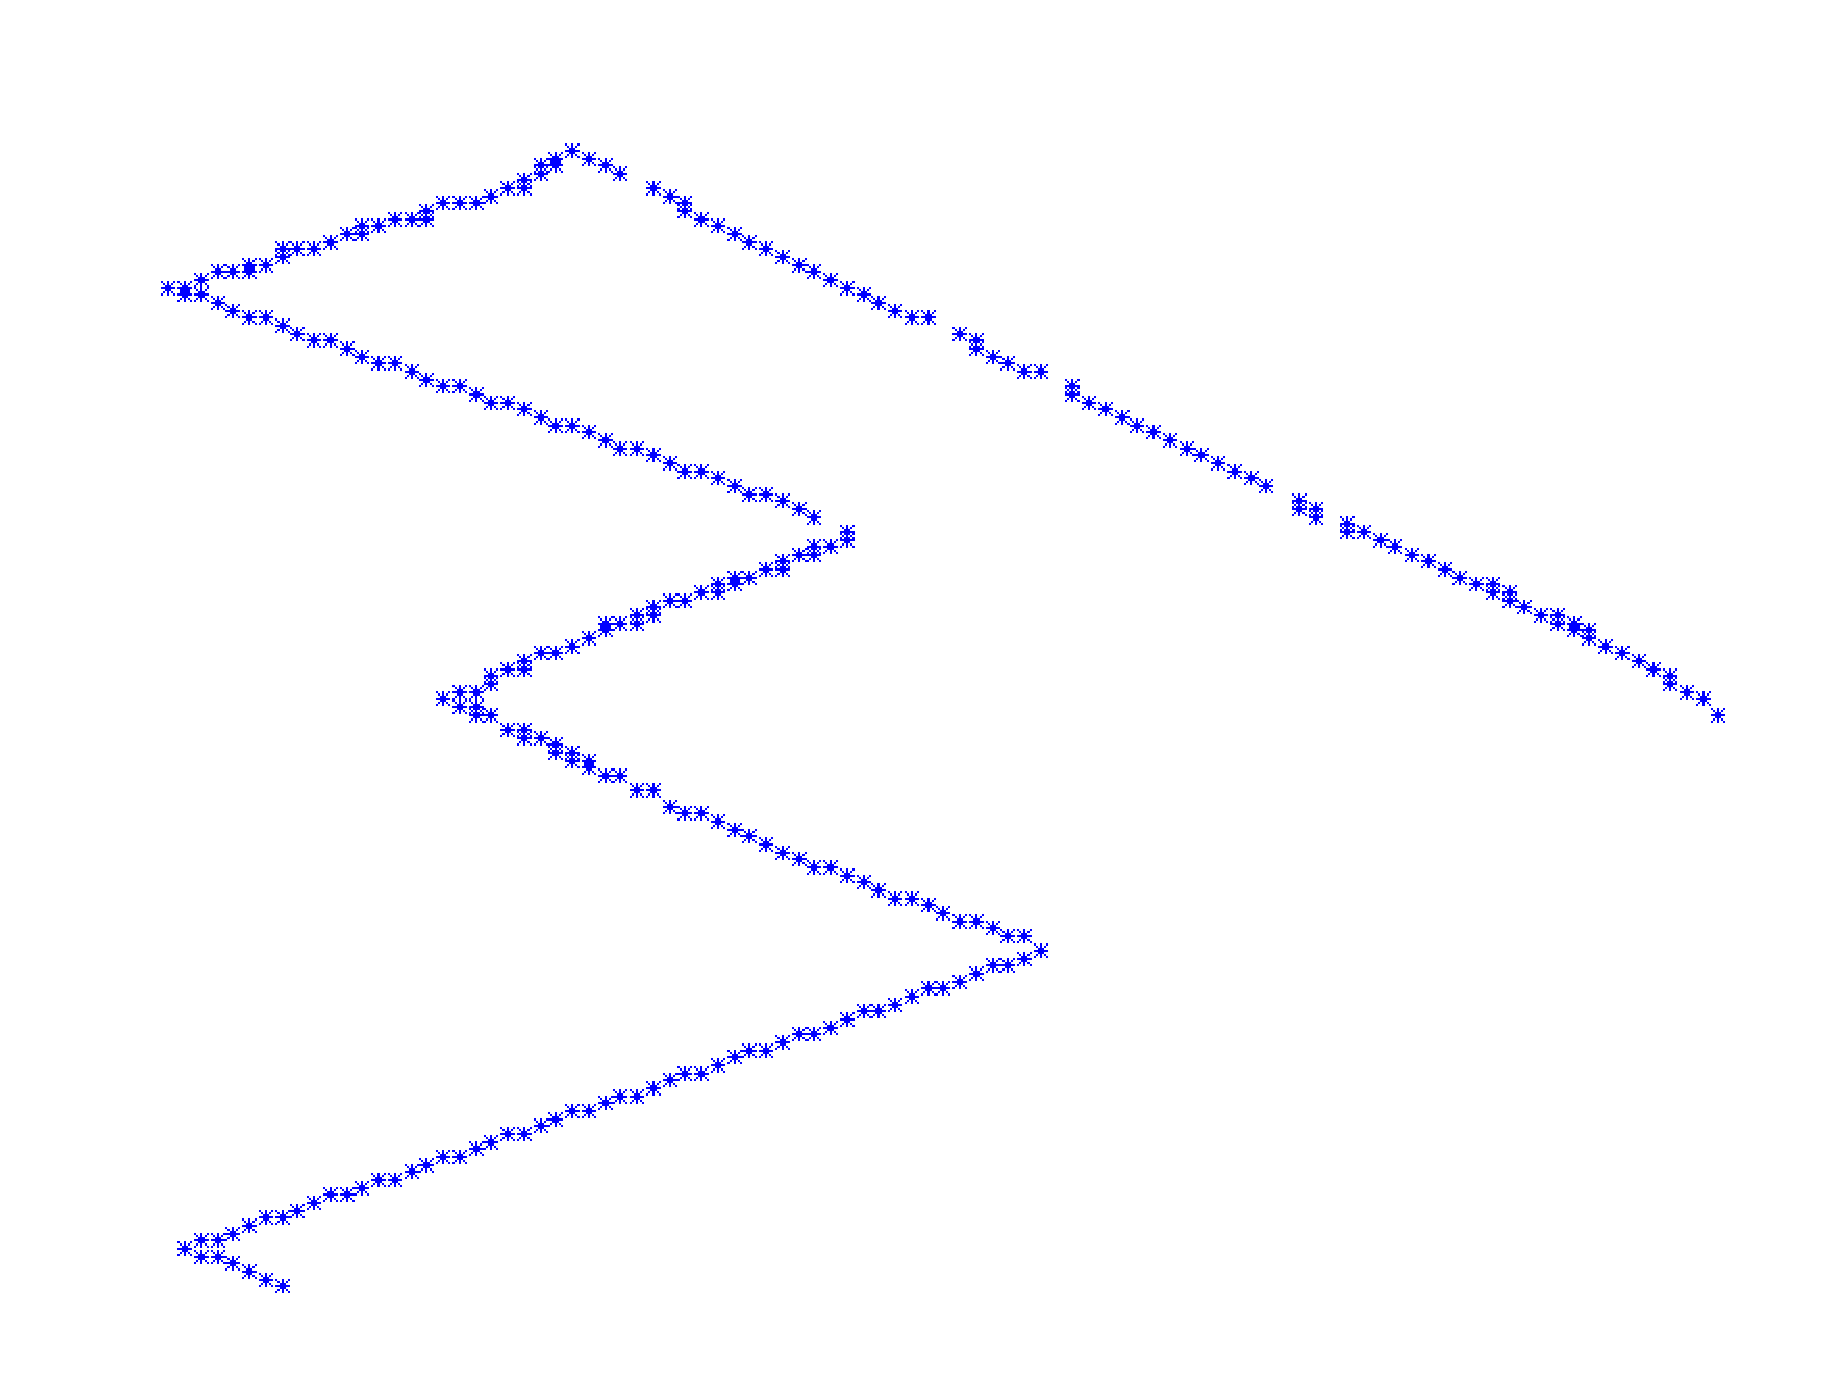
\includegraphics[width=0.4\textwidth,keepaspectratio]{images/get_line_example}
  \caption{Example of produced contour.}
	 \label{fig:get_line_example}
\end{figure}
In this step (Algorithm \ref{alg:ffd_contour_stage} lines
\ref{mark:ffd_contour_start}--\ref{mark:ffd_contour_end}) we use the
angle-sorted laser readings. The output of the contour step is a contour which
is built from the sorted laser readings. The algorithm computes the line that
lies between each two adjacent points from the set. The line is computed by
calling the function \textsc{Get-Line}. In our implementation we use
\emph{Bresenham's line algorithm} \cite{bresenham2010algorithm}. Next, all
points that are represented by all the lines (including the points from the
laser readings set) are merged into a contour (Figure \ref{fig:get_line_example}).

% 	\begin{figure}[htbp]
% 	 \centering
% 	 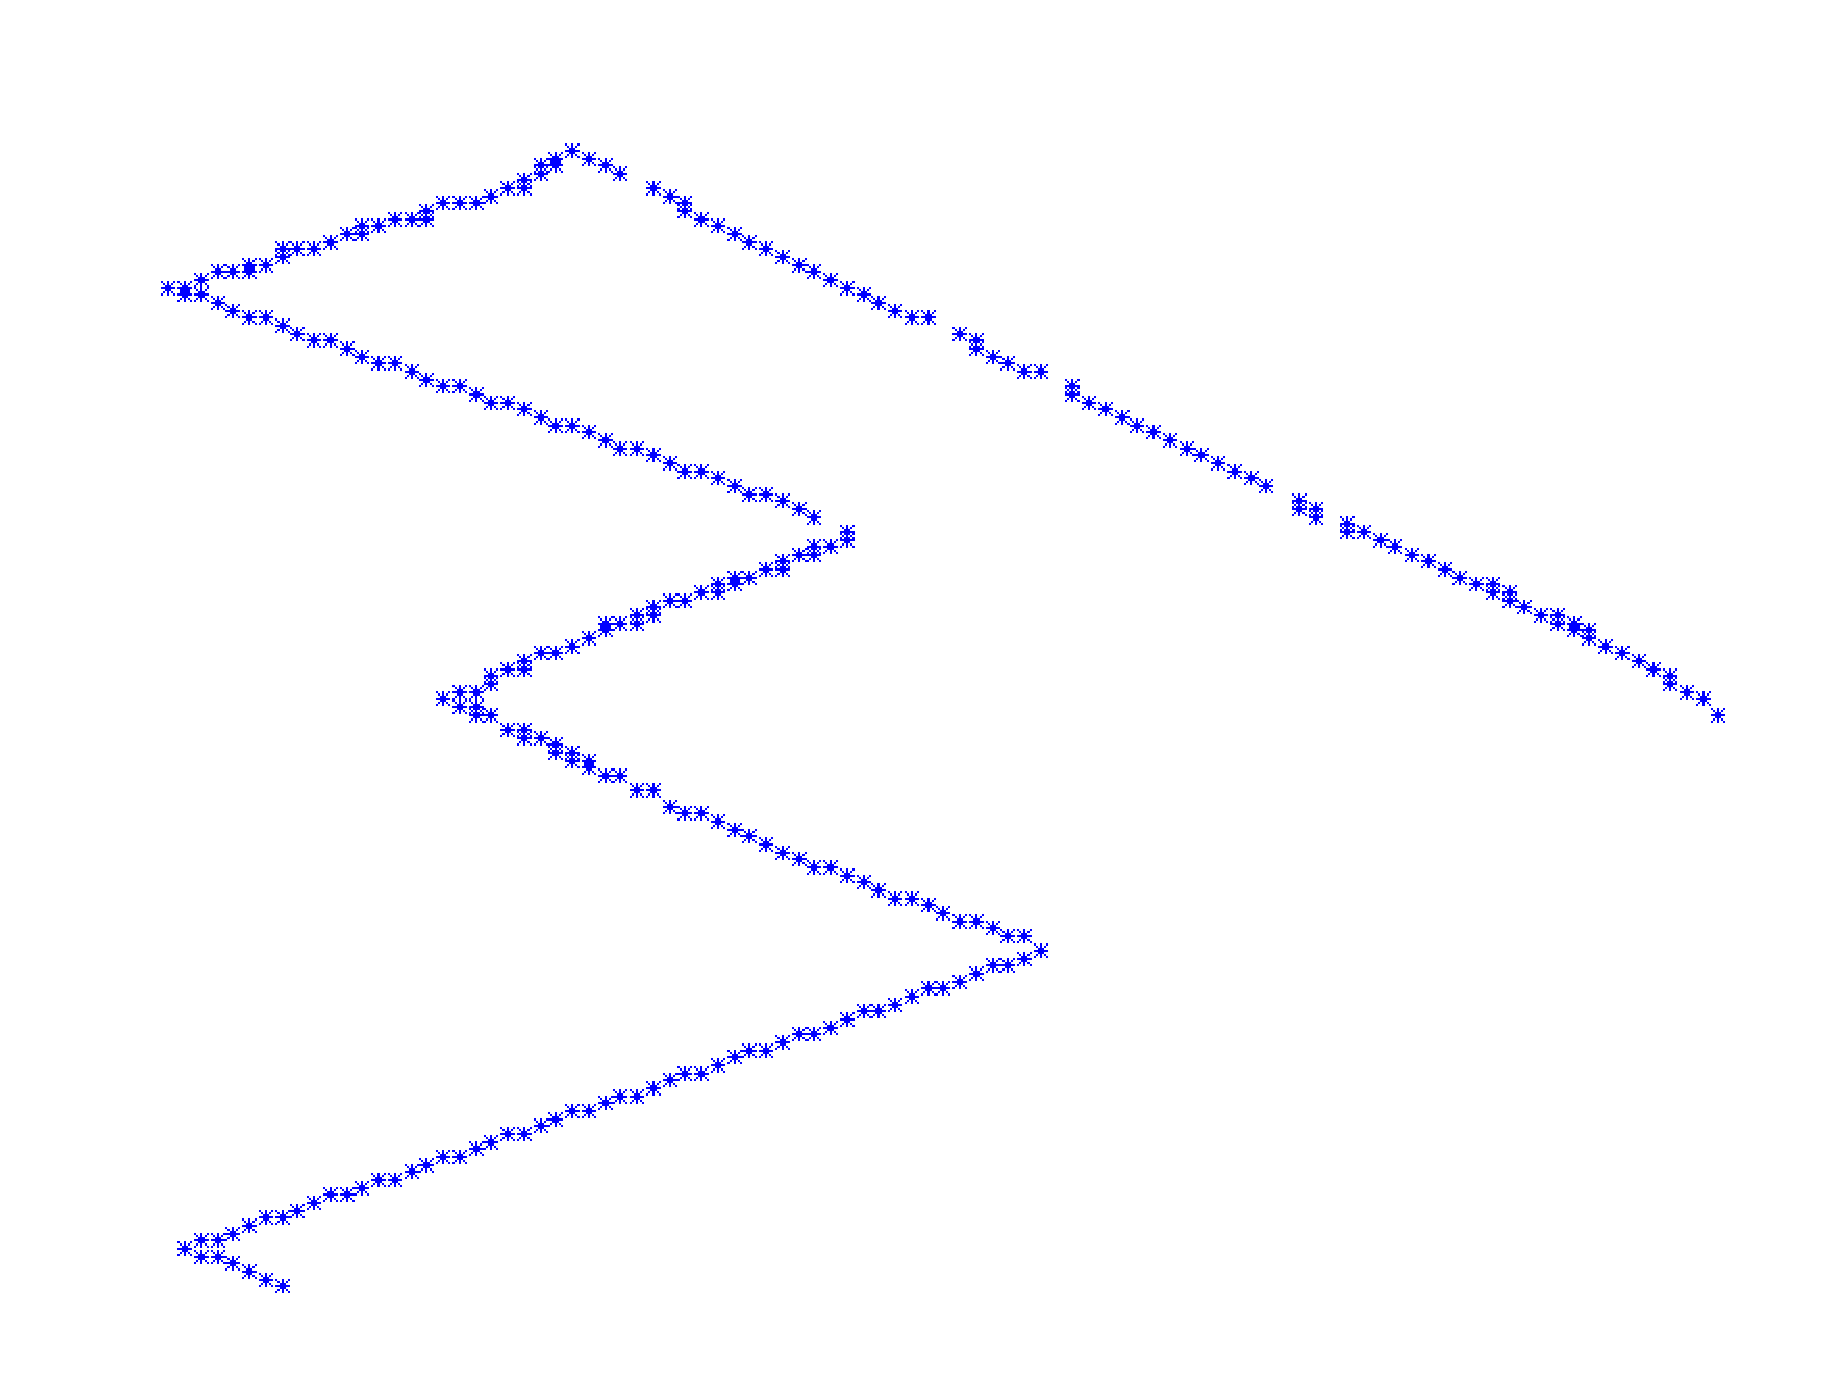
\includegraphics[width=0.4\columnwidth,keepaspectratio]{images/get_line_example}
% 	 \caption{Example of produced contour.} 	
% 	 \vspace{-15pt}
% 	 \label{fig:get_line_example}
% 	\end{figure}	



\begin{algorithm}[htbp]
\caption{Fast Frontier Detector (FFD): Extract Frontier Stage}
\label{alg:ffd_detect_new_frontier_stage}
\begin{algorithmic}[1]

\Require $contour$ 
\Comment{the contour built from the sorted laser readings}
\Ensure $NewFrontiers$
\Comment{list of new detected frontiers that lie on the contour}

\Function{Extract-Frontiers-1D}{$contour$}
\State{$NewFrontiers \gets \emptyset$} \Comment {list of new extracted
frontiers}
\label{mark:ffd_extract_start}

\State{$prev \gets POP(contour)$}

\If{$prev$ is a frontier cell} \Comment{special case}
	\State{create a new frontier in $NewFrontiers$}
\EndIf
\label{mark:ffd_special_case_end}

\ForAll {Point $curr \in contour$}
	\If {$curr$ is not a frontier cell}
	\label{mark:ffd_contour_eliminate_non_frontier_points}
		\State{$prev \gets curr$}
	\ElsIf {$curr$ has been visited before}
		\label{mark:ffd_redection_avoidance_start} 
		\State{$prev \gets curr$}
		\label{mark:ffd_redection_avoidance_end}
	\ElsIf {$curr$ and $prev$ are frontier cells}
		\State{add $curr$ to last created frontier}
		\State{$prev \gets curr$}
	\Else 
		\State{create a new frontier in $NewFrontiers$}
		\State{add $curr$ to last created frontier}
		\State{$prev \gets curr$}
	\EndIf
\EndFor 

\State \Return $NewFrontiers$
\label{mark:ffd_extract_end}
\EndFunction
\end{algorithmic}
\end{algorithm}
	\subsection{Detecting New Frontiers} \label{section:detecting_new_frontiers}
	In this step (Algorithm \ref{alg:ffd_detect_new_frontier_stage} lines
	\ref{mark:ffd_extract_start}--\ref{mark:ffd_extract_end}) the algorithm extracts new frontiers from the previously calculated contour. There are three cases correspond to each two adjacent points in the
	contour: 
	\begin{enumerate}
	\item \textbf{Current scanned point is not a frontier cell:} therefore,
	it does not contribute any new information about frontiers and can be ignored.
	
	\item \textbf{Current and previous scanned points are frontier cells:}
	therefore, both points belong to the same frontier and current scanned point is
	added to last detected frontier.
	
	% \yellownote{should we talk about that frontiers are either equal or disjoint?}
	\item \textbf{Current point is a frontier cell but the previous is
	not:} a new starting point of a frontier was detected. Hence, the algorithm creates a
	new frontier and adds the new starting point to it.
	\end{enumerate}


\begin{algorithm}[htbp]
\caption{Fast Frontier Detector (FFD): Maintenance of Previously Detected
Frontiers}
\label{alg:ffd_maintenance_stage}
\begin{algorithmic}[1]

\Require $NewFrontiers$
\Comment{list of new detected frontiers}
\Require $frontiersDB$
\Comment{data-structure that contains last known frontiers}
\Require $activeArea$
\Comment{data-structure that contains all points that lie inside the active
area}

\Function{Maintain-Frontiers}{$NewFrontiers,frontiersDB,activeArea$}

\ForAll {Point $p \in ActiveArea$}
\Comment{eliminate previously detected frontiers}
\label{mark:ffd_maintenance_start}
\label{mark:ffd_eliminating_previous_frontiers_start}
	\If {$p$ is a frontier cell} \label{mark:ffd_check_eliminate_of_frontier_point}

		\State{}		
		\Comment{split the current frontier into two partial frontiers}
		\State{get the frontier $f \in frontiersDB$ which enables $p \in f$}
		\label{mark:ffd_split_frontier_start}	
		\State{$f_1 \gets f[1\ldots p]$}
		\label{mark:split_start}
		\State{$f_2 \gets f[(p+1)\ldots |f|]$}
		\label{mark:split_end}
		\State{remove $f$ from $frontiersDB$}
		\State{add $f1$ and $f2$ to $frontiersDB$}
		\label{mark:ffd_split_frontier_end}
	\EndIf
\EndFor
\label{mark:ffd_eliminating_previous_frontiers_end}


\ForAll {Frontier $f \in NewFrontiers$}
\Comment{store new detected frontiers}
\label{mark:ffd_storing_new_frontiers_start}
	\If {$f$ overlaps with an existing frontier $ExistFrontier$}
		\State{$merged \gets f \cup ExistFrontier$}
		\State{remove $ExistFrontier$ from $frontiersDB$}
		\State{add $merged$ to $frontiersDB$}
	\Else 
		\State{create a new index and add $f$ to $frontiersDB$}	
	\EndIf
\EndFor
\label{mark:ffd_storing_new_frontiers_end}
\label{mark:ffd_maintenance_end}
\EndFunction
\end{algorithmic}
\end{algorithm}
	 
	\subsection{Maintaining Previously Detected
	Frontiers}\label{section:ffd_maintaining_previously_detected_frontiers} \FFD
	gains its speed by processing the laser readings only, rather than entire regions of the map.
	However, if the robot navigates towards a specific frontier, other previously
	detected frontiers are no longer updated because they are not covered by
	the robot's sensors. Thus, scanning the new received laser readings enables
	\FFD to detect only \emph{new} frontiers in each execution. In this step
	(Algorithm \ref{alg:ffd_maintenance_stage} lines
	\ref{mark:ffd_maintenance_start}--\ref{mark:ffd_maintenance_end}), in order to
	get complete information about the frontiers, the algorithm performs
	maintenance over previously detected frontiers which are no longer covered in
	the range of the sensors. Only by joining together new detected frontiers and
	previously detected frontiers, we get the overall frontiers in current world
	state. This step has multiple goals: avoiding detection of new frontiers in
	an already scanned area (Section \ref{section:avoiding_redetection}),
	eliminating frontier points which are no longer belong to frontiers (Section
	\ref{section:frontier_elimination}) and joining correctly the new detected
	frontiers together with previously detected frontiers (Section
	\ref{section:storing_frontiers}).
		
	
% 	\FFD requires the previously detected frontiers to be robust against
% 	map orientation changes caused by loop-closures of the mapping algorithm.
% 	In a \emph{Particle Filter} based SLAM infrastructures, changes in active
% 	particles probably occur. Hence, because particles do not share maps,
% 	each particle runs its own instance of \emph{FFD}.
	
% 	\subsubsection{Kalman Filter}
% 	The situation is different in \emph{Extended Kalman-Filter} (EKF) based SLAM
% 	infrastructures. These infrastructures have one map that is updated.
% 	Hence, data can be stored within a map in EKF SLAM infrastructures because the
% 	information about changing map orientation is available (in contrast to
% 	particle-based systems in which every particle is independent from the other
% 	particles).
	
	%EKF implementation contains one map which is updated by
	%the mapping algorithm (rather than several maps in Particle-Filter based SLAM
	%implementation)

	\subsubsection{The \FFD Data-Structures}
	In order to perform the maintenance step within a very short time as possible,
	\FFD utilizes two data-structures which have a short access time.  These data structures
        must maintain memory of frontiers between calls. Thus \FFD has to have persistent memory,
        i.e., data structures that persist between calls. This is contrast to
        other approaches that can be executed in a certain time, and only then. 

	Another thing to note is that in particle filter based systems (our focus in
	this thesis), each particle represents a possible hypothesis of the world state
	(including the robot position of course). The ``best'' particle is chosen
	according to a likelihood measurement. \FFD requires the previously detected
	frontiers to be robust against map orientation changes caused by loop-closures
	of the mapping algorithm.
	Therefore, when a new laser reading is received, \emph{each} particle executes
	its own instance of \FFD algorithm on its own map, using its own data structures. More
	specifically, each particle performs maintenance with its own map because
	particles do not share maps.
	We describe the data structures for maintenance below.
	
The first, \emph{Grid of Frontier Indices}, is an extension
of the occupancy grid (though it can be implemented as a separate entity). In
addition to occupancy information, each grid cell contains \textit{a frontier
index}, pointing to a frontier to which the grid cell belongs, or NULL
otherwise. The pointer points to a record stored in the Frontier Database
(described below).
In our implementation, we used integer index values. After accessing a grid cell
(Algorithm \ref{alg:ffd_maintenance_stage} Line
\ref{mark:ffd_check_eliminate_of_frontier_point}), querying for its frontier
index is $O(1)$.
	
	
% 	This data structure is a simple table in
% 	size of the grid which represents the world. Each cell contains either NULL,
% 	which represents that the cell is not a frontier cell, or an integer value,
% 	which represents that the cell is a frontier cell and belongs to the frontier
% 	whose index is that integer value. Using this grid of frontier indices
% 	enables us to quickly query wether a specific point in the world has been
% 	already declared as a frontier point. In our implementation, we expanded each
% 	map cell to have an additional attribute for storing its frontier index or
% 	NULL. Therefore, we could reuse the world map as the grid of frontier
% 	indices. After accessing a map cell, quering its frontier index is $O(1)$.
	
	The second, \emph{Frontier Database}, maps frontier
	indices (pointers) to sets of points ($frontierDB$ requirement of Algorithm
	\ref{alg:ffd_outline} and Algorithm \ref{alg:ffd_maintenance_stage}).
	All detected frontiers are stored in this data-structure. We use it to map frontier index to the actual set that
	contains the points in world coordinates. In our implementation, we use the
	default C++ implementation of a map template, which is implemented as a
	self-balancing binary search tree.
	Therefore, assuming $n$ represents the number of frontiers stored in the
	database, searching for a frontier index takes $O(\log n)$, inserting a new
	frontier takes $O(\log n)$ and removing a frontier index takes $O(\log n)$,
	though a (hash) table lookup implementation can make this faster.
	% XXX Matan, am I wrong about the hash table lookup?

	\subsubsection{Avoiding Re-Detection of Same Frontier}
	\label{section:avoiding_redetection}
	\FFD detects new frontiers by processing laser readings only.
	Hence, \FFD might detect the same frontier again and classify it as a new
	frontier if the robot did not change its position during two following \FFD
	executions. Moreover, if the robot travels back to an already visited
	region, no new frontiers should be detected. \FFD has to distinguish between
	laser readings from  between time frames. Otherwise, \FFD might wrongly detect
	a new frontier which lies within an already scanned area.

	Therefore, we keep track of the number of sensor visits (sensor covers) of each map cell. The
	definition of a frontier point is now expanded: a frontier point is a point
	which represent an unknown region, has at least one open-space neighbor and has
	not been scanned before. Given a contour, the detection of new frontiers ignores
	points that have already been scanned by the laser sensors and treats them as
	non-frontier points (Algorithm \ref{alg:ffd_detect_new_frontier_stage} lines
	\ref{mark:ffd_redection_avoidance_start}--\ref{mark:ffd_redection_avoidance_end}).

	Figure \ref{fig:redetecting_examples} demonstrates the necessity of the above.
	Figure \ref{fig:redetecting_bad} shows frontiers extraction
	without tracking the number of visits. It can be seen that there are frontiers that lie inside
	an open space area. This is absolutely wrong because frontiers are supposed to
	be positioned on the boundaries between known and unknown regions. In
	contrast, Figure \ref{fig:redetecting_good} shows frontiers extraction with
	avoidance of re-detecting same frontiers. It can be seen that every frontier
	separates known and unknown regions.
	
	\begin{figure}
	 \centering
	 \subfigure[Incorrectly re-detected frontiers.] {
	 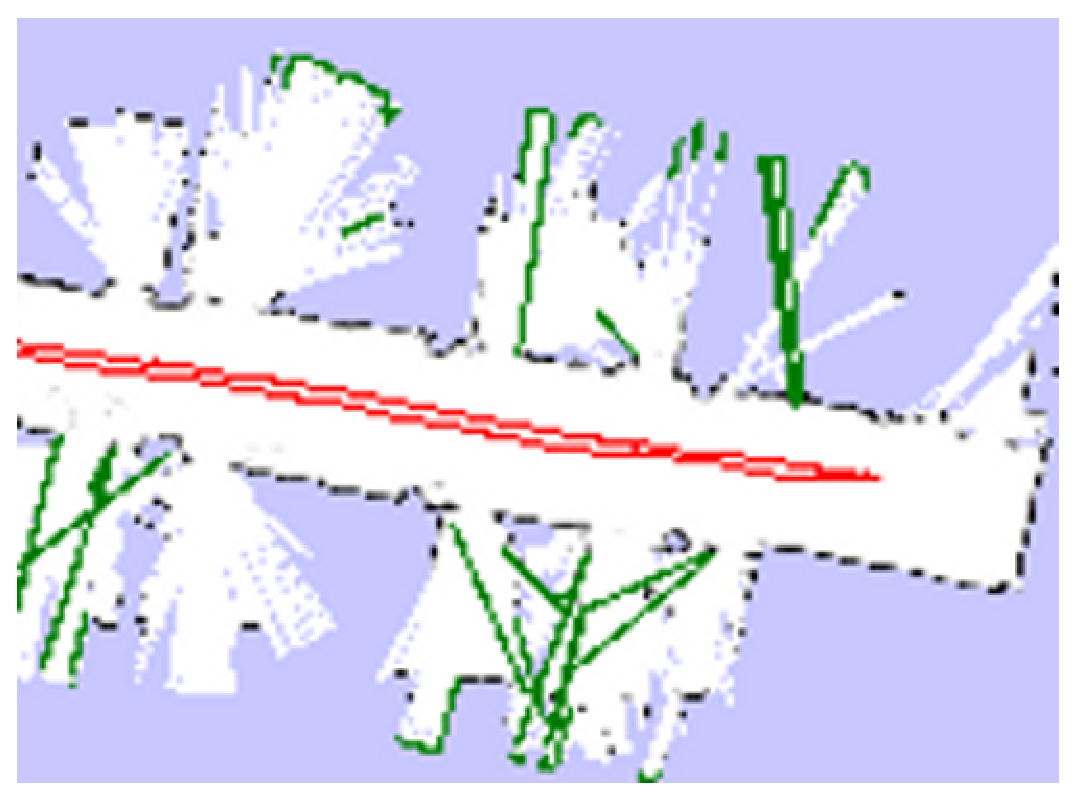
\includegraphics[width=0.47\columnwidth,keepaspectratio]{images/redetecting_bad_example.eps}
	 \label{fig:redetecting_bad}}
	 \subfigure[Correct detection.] {
	 \centering
	 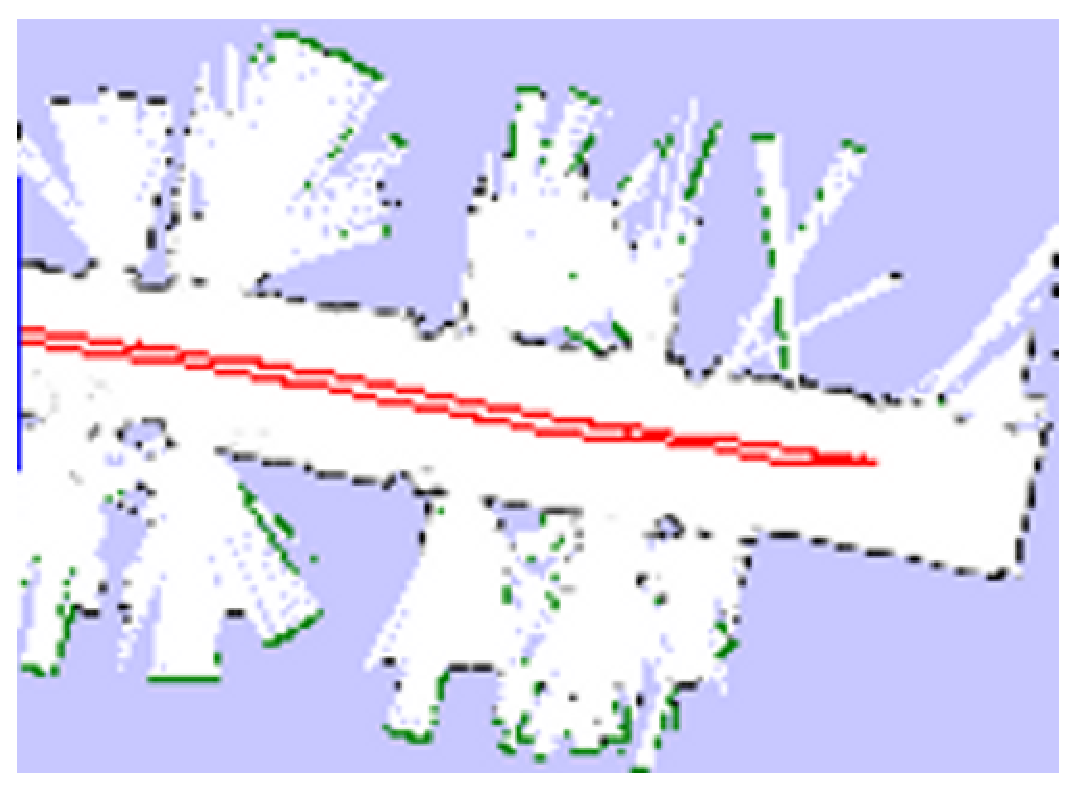
\includegraphics[width=0.47\columnwidth,keepaspectratio]{images/redetecting_good_example.eps}
	 \label{fig:redetecting_good}}
	 \caption{An example of re-detecting same frontiers.}
	 \label{fig:redetecting_examples}
	\end{figure}

	\subsubsection{Eliminating Previously Detected Frontiers}
	\label{section:frontier_elimination}
	In order to complete the process, points which are no longer in frontiers  (i.e. were
	covered by the robot's sensors) have to be eliminated. Lines
	\ref{mark:ffd_eliminating_previous_frontiers_start}--\ref{mark:ffd_eliminating_previous_frontiers_end}
	in Algorithm \ref{alg:ffd_maintenance_stage} contain the elimination logic
	applied by \FFD.

	%\paragraph{Active Area} 
	Let $t_i$ be a time frame and $lr_{t_i}$ be the laser readings which
	were received in time frame $t_i$. In order to perform maintenance in a specific
	time, we define the \emph{Active Area} of time frame $t_i$ to be the blocking
	rectangle that can be constructed using the farthest laser readings of
	$lr_{t_i}$, relative to the robot position in time frame $t_i$. 
	$$ x_{min} = min(\left\{x | x \in lr_{t_i} \right\}) ,
	 y_{min} = min(\left\{y | y \in lr_{t_i} \right\}) $$ 
	$$ x_{max} = max(\left\{x | x \in lr_{t_i} \right\}) ,
	 y_{max} = max(\left\{y | y \in lr_{t_i} \right\}) $$ 
	$$ActiveArea_{t_i} = \left\{\left(x,y \right) | x_{min}  \leq x \leq x_{max} ,
	y_{min}  \leq y \leq y_{max} \right\}$$ 
	The active area's rectangle is constructed from the following vertices: 
	$\left(x_{min},y_{min} \right)$,
	        $\left(x_{min},y_{max} \right)$,
	        $\left(x_{max},y_{max} \right)$,
	        $\left(x_{max},y_{min} \right)$. 
	The rectangle is an approximation to the real active area that is actually
	bounded within the laser readings. 
	%In the following section, we will explain
	%why the active area is a key feature in the process of maintaining frontiers.

% 	\subsubsection{Frontier Elimination}
	By processing received laser readings, \FFD extracts new frontiers.
	However, in order to get the complete world's frontiers state, points
	that are no longer on frontiers have to be eliminated. \FFD maintains a frontier
	database which maps an integer (frontier index) to a set of points (frontier).
	
	An unknown region is classified as known region only if it is covered by the
	robot's sensors. \FFD gets its input from the new received
	laser readings, and thus only regions that are covered by the
	robot's sensors might contain frontiers that have to be eliminated. Thus, if there are frontiers that need to be eliminated, they must
	lie inside the \emph{Active Area}. Hence, the active area is a key feature
	in the process of maintaining frontiers. \FFD scans each point that lies inside
	the active area and checks if it was previously belonged to a frontier. The
	check can be performed very fast as explained before. If the current scanned
	point was belonged to a frontier, the current scanned point is removed from
	the frontier and the frontier is splitted into two partial frontiers using the
	current scanned point as a pivot (Algorithm \ref{alg:ffd_maintenance_stage} lines
	\ref{mark:split_start}--\ref{mark:split_end}).
 
	In the end of this process, all no-longer frontier points in the frontier
	database are removed and the database contains only points that are still valid
	frontiers. 
	
	\subsubsection{Storing New Detected Frontiers}
	\label{section:storing_frontiers}	
	In the last phase of the maintenance step (Algorithm
	\ref{alg:ffd_maintenance_stage} lines
	\ref{mark:ffd_storing_new_frontiers_start}--\ref{mark:ffd_storing_new_frontiers_end})
	new detected frontiers are stored in the frontier database alongside with
	existing valid frontiers.  For each new detected frontier, \FFD checks if it
	overlaps with an already existing frontier. This comparison can be performed
	in a short time using the matrix of frontier indices. Each frontier point is
	queried in $O(1)$ operations. If an overlap is found, the frontier is merged
	with the frontier that it is overlapped with. If no overlap is found, then the
	frontier is inserted to the frontier database.
	
	
% 	We find \emph{Kalman-Filter} (EKF) based SLAM implementations best for
% 	integrating \FFD. In Section \ref{section:future_work}, we suggest a solution to
% 	integrate \FFD into Particle-Filter based SLAM implementations.
	
%\end{description}

% \input{algorithms/getContour} \input{algorithms/extractFrontiers}

% \yellownote{need to implement maintenance part of FFD}


\section{\FFD is Sound and Complete}
\label{section:ffd_sound_and_complete}
% \subsection{Completeness}
We show that Algorithm~\ref{alg:ffd_outline} is sound and complete.
We begin with a lemma that demonstrates that \FFD always recognizes new
frontiers (i.e., frontiers that appeared at time $t$, but did not exist before).
This will then be used to prove completeness of \FFD.
% \vspace{-7pt}
\begin{lemma}
\label{lem:newf}
Suppose $f$ is a frontier point at time $t$, which was not a frontier point at
any time $s$, where $s<t$. Then FFD will mark $f$ as a frontier given
observation $O_t$.
\end{lemma}
% \vspace{-10pt}
\begin{proof}
Let $f$ be a valid frontier point in time $t$ and was not classified as
frontier in time $s<t$. Since $f$ is a valid frontier point, then it has a
value of \emph{Unknown} and has at least one \emph{Open Space} neighbor at time
$t$. 
Assume towards a contradiction that \FFD did not recognize $f$ as a frontier
point. First, let us show that $f$ is contained in the contour handled
in Algorithm \ref{alg:ffd_detect_new_frontier_stage} lines
\ref{mark:ffd_extract_start}--\ref{mark:ffd_extract_end}.
Since $f$ is a valid frontier point, then it has a value
of \emph{Unknown} and has at least one \emph{Open Space} neighbor in time
$t$. The point $f$ cannot be located wholly within an \textit{unknown} region because it must
have at least one \emph{Open Space} neighbor. Also, the point $f$ cannot be
located wholly within a \textit{known} region since $f$ is a valid frontier point and
hence, its value is $Unknown$. Therefore, $f$ must be located on the contour
itself.
Lines \ref{mark:ffd_extract_start}--\ref{mark:ffd_extract_end} in Algorithm
\ref{alg:ffd_detect_new_frontier_stage} handle points on the contour, which we
have just shown $f$ is on. In these lines, the \FFD algorithm scans \emph{all}
contour points sequentially and specifically searches for frontier points.
Because it scans \emph{all} points on the contour, and we have shown that $f$
is on the contour, it follows that $f$ would be detected, contradicting the
assumption that \FFD did not recognize $f$ as a frontier point at time $t$.
\end{proof}
%\end{comment}

We now turn to proving the completeness of the \FFD algorithm. 
\begin{theorem}
 \label{thm:complete}
Let $f$ be a valid frontier point at time $t$. Then FFD will mark $f$ as a frontier point
given the sequence of observations $\langle O_0,\ldots,O_t\rangle$.
\end{theorem}

\begin{proof}
Two cases should be examined:

\noindent{\bf Case 1. $f$ is a new frontier point at time $t$.} Trivially,
this case is handled directly by lemma \ref{lem:newf}.

\noindent{\bf Case 2. $f$ was a new frontier point at time $s$, where $s<t$.}
Let $s$ be the earliest time in which $f$ was a frontier. Based on lemma 
\ref{lem:newf}, it follows that it was detected at this time. All that  remains
to show is that given $f$ is still valid at time $t$, \FFD will maintain
knowledge of it from time $s$ and report on it.
If $f$ is still a valid frontier point at time
$t$, then it has not been covered yet by the robot's sensors. Otherwise, it
would  no longer contain an \emph{Unknown} value and hence, would not
be a valid frontier point.  
So if it was not yet covered, it must be a frontier point that is maintained by 
\FFD. The only way in which $f$ can be eliminated from  being classified
as a frontier point is done by Algorithm \ref{alg:ffd_maintenance_stage} lines
\ref{mark:ffd_eliminating_previous_frontiers_start}--\ref{mark:ffd_eliminating_previous_frontiers_end}.
In these lines, \FFD scans all points that are covered by the robot's sensors
and checks if any points should be eliminated (Algorithm
\ref{alg:ffd_maintenance_stage} line
\ref{mark:ffd_check_eliminate_of_frontier_point}). Since $f$ is not covered by
the sensors, then it will not be scanned and eliminated in time $t$
$\Rightarrow$ $f$ remains classified as a frontier by \FFD.


In both cases we show \FFD will recognize $f$ to be a valid frontier at time $t$.
Since Theorem \ref{thm:complete} is true for any frontier point valid at time $t$,
it follows that \FFD is complete.   
\end{proof}
%\end{comment}


% \subsection{Soundness}
To show the soundness of \FFD, we must demonstrate that there does not exist a case
where \FFD marks a point $\hat{f}$ as a frontier, when it is not.

\begin{theorem}
\label{thm:sound}
Let $\hat{f}$ be an arbitrary point in the occupancy grid, which is \emph{not}
a frontier at time $t$. Then FFD will not return $\hat{f}$ as a frontier point,
given the sequence of observations $\langle O_0,\ldots,O_t\rangle$.
\end{theorem}

\begin{proof}
Assuming that $\hat{f}$ is an arbitrary point which is \emph{not} a frontier
point at time $t$, then $\hat{f}$ is either contains value different from
\emph{Unknown} or all its adjacent values are different from \emph{Open
Space}. We will examine two cases:

\noindent{\bf Case 1. $\hat{f}$ is marked as a new frontier.}
Suppose, towards a contradiction, that \FFD detects $\hat{f}$ as a new frontier
(i.e., true at time $t$, but not a frontier in time $s$, where $s<t$).
Since detection of new frontier points (Algorithm \ref{alg:ffd_detect_new_frontier_stage} lines
\ref{mark:ffd_extract_start}--\ref{mark:ffd_extract_end}) considers only points
on the contour, it follows that $\hat{f}$ must be located on the contour
\emph{and} detected by Algorithm \ref{alg:ffd_detect_new_frontier_stage} lines
\ref{mark:ffd_extract_start}--\ref{mark:ffd_extract_end}. However, Algorithm
\ref{alg:ffd_detect_new_frontier_stage} line \ref{mark:ffd_contour_eliminate_non_frontier_points}
specifically avoids classifying non-frontier points as frontiers. Since $\hat{f}$ is a non-frontier
point, it is ignored by \FFD. Therefore, $\hat{f}$ cannot be marked as a new
frontier $\Rightarrow$ contradicting the assumption that it is detected by \FFD
as a new frontier. Case 1 is impossible.

\noindent{\bf Case 2. $\hat{f}$ is an old frontier but was not
eliminated by the maintenance routine.} Suppose, towards a contradiction, that $\hat{f}$ is
located inside the active area and is not eliminated by the maintenance section.
Therefore, $\hat{f}$ is a point that was covered by the robot's sensors and no
longer contains an \emph{Unknown} value, yet is still marked as a frontier by
the \FFD algorithm.
We remind the the reader that in order to maintain frontier points across runs,
each point in the grid keeps a value which contains NULL if the point is not a
frontier point or the index of the frontier to whom it belongs.
Therefore, in Algorithm \ref{alg:ffd_maintenance_stage} line
\ref{mark:ffd_check_eliminate_of_frontier_point} \FFD scans all points in the
active area and checks if they contain a frontier index. When \FFD scans
$\hat{f}$, it finds out that it contains a valid frontier index (because it
has previously belonged to a valid frontier) and continues executing
Algorithm \ref{alg:ffd_maintenance_stage} lines
\ref{mark:ffd_split_frontier_start}--\ref{mark:ffd_split_frontier_end}. In
these lines, \FFD checks and removes from the frontier database all points that
are no longer frontier points and previously were frontier points. Thus,
$\hat{f}$ will be eliminated after scanning the active area, contradicting the
assumption that $\hat{f}$ was not eliminated.

Since in both cases we show that \FFD necessarily eliminated $\hat{f}$ from the
valid frontier list, it follows that if $\hat{f}$ is not a frontier-point at time $t$, it would not
be marked as such by \FFD.
Since Theorem \ref{thm:sound} holds for any arbitrary point, it follows that
\FFD never incorrectly marks a non-frontier point as a frontier. It is thus
sound.
\end{proof}
%\end{comment}

